\documentclass{article}


\usepackage{lipsum}
\usepackage[margin=1in,includefoot]{geometry}
\usepackage{graphicx}
\usepackage{float}
\usepackage[hidelinks]{hyperref}
\usepackage{amsmath}
\usepackage{amssymb}
\usepackage{color}
\usepackage[english]{babel}
\usepackage{subcaption}

\usepackage{booktabs}
\usepackage[normalem]{ulem}
\useunder{\uline}{\ul}{}

\usepackage[usenames,dvipsnames]{xcolor}
\usepackage{listings}


% Header and Footer Stuff
\usepackage{fancyhdr}
\pagestyle{fancy}
\fancyhead{}
\fancyfoot{}
\fancyfoot[R]{\thepage}
\renewcommand{\headrulewidth}{0pt}
\renewcommand{\footrulewidth}{0pt}




\definecolor{dkgreen}{rgb}{0,0.6,0}
\definecolor{gray}{rgb}{0.5,0.5,0.5}
\definecolor{mauve}{rgb}{0.58,0,0.82}


\lstset{
 language=C++,
 aboveskip=3mm,
 belowskip=3mm,
 showstringspaces=false,
 columns=flexible,
 basicstyle={\small\ttfamily},
 numbers=none,
 numberstyle=\tiny\color{gray},
 keywordstyle=\color{blue},
 commentstyle=\color{dkgreen},
 stringstyle=\color{mauve},
 breaklines=true,
 breakatwhitespace=true,
 tabsize=3
}




\begin{document}


\begin{titlepage}
	\begin{center}
	\begin{align*}
	
\includegraphics[height=1.75in]{logo.png}
	\end{align*}




	
	\line(1,0){300}\\
	[0.25in]
	\huge{\bfseries Road Sign Preprocessing}\\
	[2mm]
	\line(1,0){200}\\
	[1.5cm]
	\textsc{\LARGE Assignment 1}\\
	[0.75cm]
	\textsc{\Large CS4053 Computer Vision}\\
	[7cm]	
	\end{center}
	
	
	
	\begin{flushright}
	\textsc{\large Alexandru Sulea\\
	D Stream\\
	\#12315152\\
	30 Octomber 2016\\}
	\end{flushright}
	
\end{titlepage}
%Table of Contents Stuff%
\tableofcontents
%\listoffigures
%\addcontentsline{toc}{section}{List of Figures}
\listoftables
\addcontentsline{toc}{section}{List of Tables}




\thispagestyle{empty}
\cleardoublepage
\pagenumbering{arabic}
\setcounter{page}{1}


\pagebreak
\section{RED PIXEL DETECTION}
\subsection{Intro}\label{sec:intro}
In this section the procedures and results for detecting red pixels are outlined. For this part of the assignment the lecture notes, recommended reading and online openCV recources were used to plan an adequate procedure for completing the assignment.\\
\begin{lstlisting}




\end{lstlisting}
\subsection{Procedure}\label{sec:intro}
Taking notes of what was discussed and shown in class together with online forms and the opencv page, I chose to plan out my procedure based on a histogram and backprojection detection model.
To use the histogram though, red samples were needed to, in essence teach the opencv program what red is, and more specifically what type of red was required to be recognised for the assignment.\\
The histogram could not be constructed out out of the unaltered sample picture provided due to the program not understanding what it was required to look for.A histogram needs to be instructed what type of data to look for.\\
A histogram is a collected count of data, the data is not limited to color hue, the data can be anything from intensity values to gradients and directions. The histogram for this tutorial was chosen to only count the hue. This decision was taken due to the objective of the assignment was to find different road signs, all of which had a red contour. Thus the easiest way to find red is to search for all the ranges of the red hue included in road 
signs.
\begin{figure}[H]
\begin{subfigure}{0.5\textwidth}
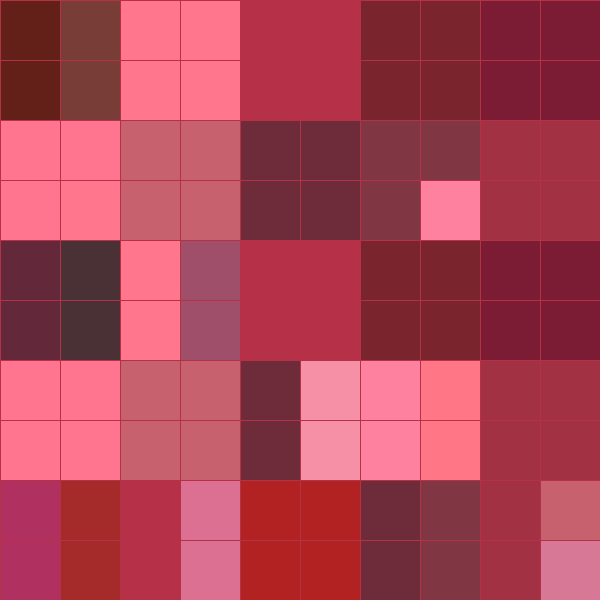
\includegraphics[width=0.9\linewidth, height=5cm]{ROADSIGN_samplered.png} 
\caption{The second last red sample}
\label{fig:subim1}
\end{subfigure}
\begin{subfigure}{0.5\textwidth}
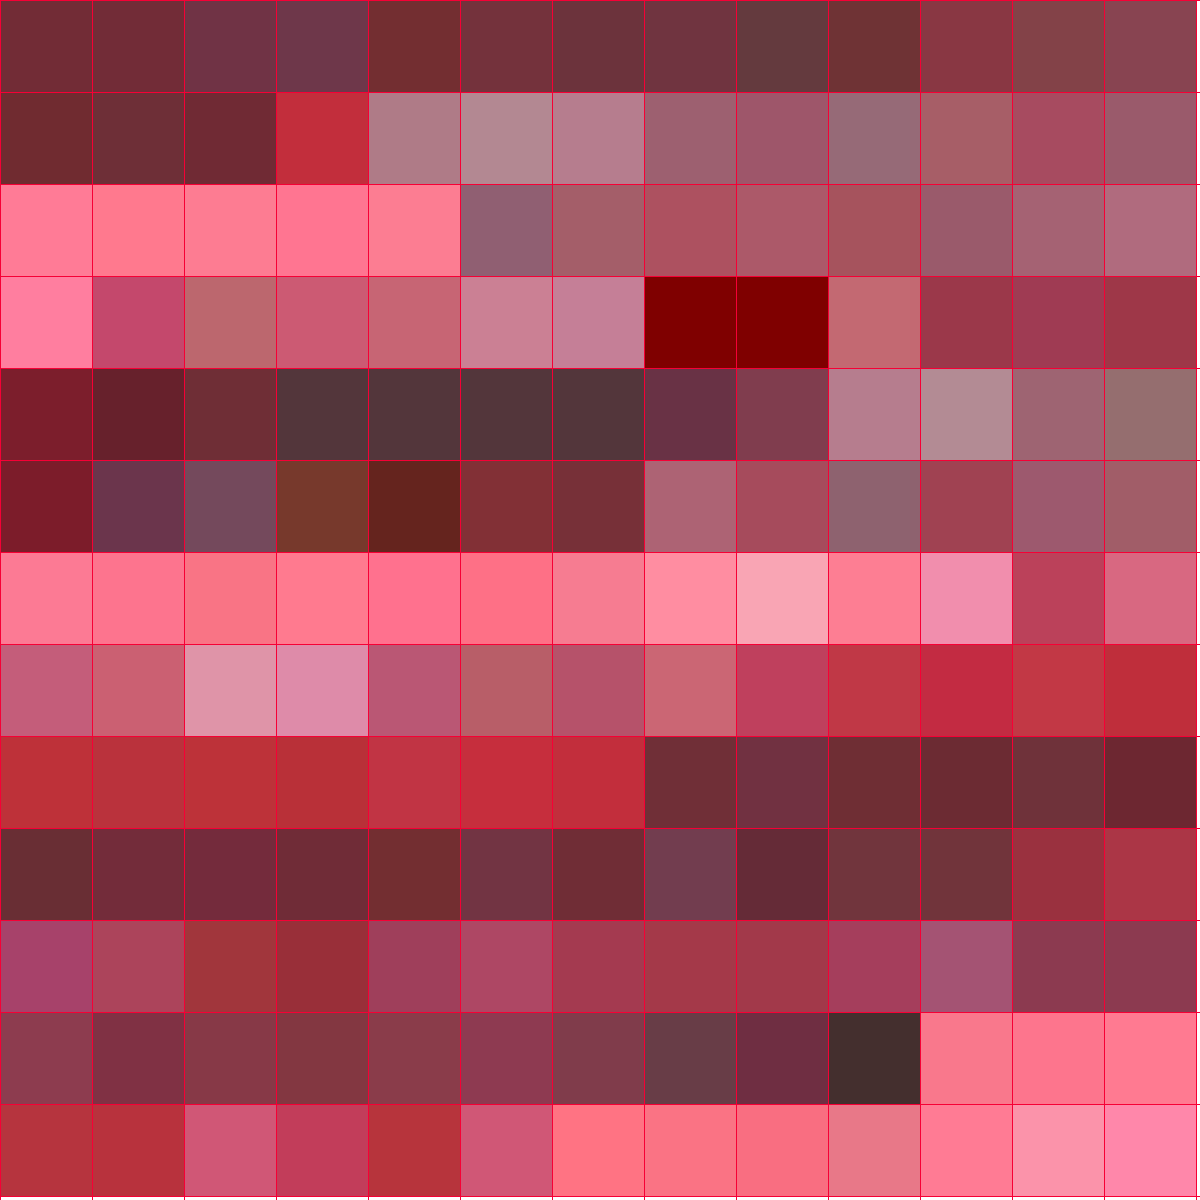
\includegraphics[width=0.9\linewidth, height=5cm]{ROADSIGN_samplered2.png}
\caption{The red sample image used for the current results}
\label{fig:subim2}
\end{subfigure}
\caption{Figure of constructed red sample images}
\label{fig:image2}
\end{figure}
Thus, a new sample red image had to be created to make a histogram which would only contain the red present in road signs. To make the red sample image  the photoshop program gimp was used to make a simple grid in which different red hues were stored. The red hue samples were taken from the sample road signs image. The images road signs were sampled at different points so as to get an even, accurate representation of the red color used in the road signs.\\
Once the new sample red image had been created using different points on road signs in the sample road signs image the code could finally be written in.\\
The first step is to load in the images and check that the correct images have been loaded by the program without any exceptions or errors being thrown. That is where this part of the code comes in.
\begin{lstlisting}
Mat roadsign_test2 = imread("filename.JPG", CV_LOAD_IMAGE_UNCHANGED);
if (roadsign_sample.empty()){
		printf("Cannot open video file: \n");
		return -1;}
	else { ...}
\end{lstlisting}
Next the image is converted to HSV or Hue Saturation Value so that we can separate the hue from the rest of the image. Since we are only interested in the color red and its multiple shades we will only be using hue, thus creating a 1D Red Hue Histogram.


\begin{lstlisting}
//hue is from 0 to 180
		float huerange[] = {0, 180};
		//use only hue value
		hue_red.create(hsv_sample_red.size(), hsv_sample_red.depth());
		mixChannels(&hsv_test, 1, &hue_test, 1, ch, 1);
		/*Calculate and Normalize Hist*/
		calcHist(&hue_red, 1, ch, Mat(), hist_red, 1, &histSize_red, &ranges, true, false);
		normalize(hist_red, hist_red, 0, 255, NORM_MINMAX, -1, Mat());
		//drawing out the red histogram
		Mat histImg = Mat::zeros(w, h, CV_8UC3);
		for (int i = 0; i < bins; i++)
		{
			rectangle(histImg, Point(i*bin_w, h), Point((i + 1)*bin_w, h - cvRound(hist_red.at<float>(i)*h / 255.0)), Scalar(0, 0, 255), -1);}
		calcBackProject(&hue_test, 1, 0, hist_red, backproj, &ranges, 1, true);	
		threshold(backproj, thresh_backproj, 8, 255, CV_THRESH_BINARY);
		dilate(thresh_backproj, dil_thresh_backproj, Mat(), Point(-1, -1), 2, 1, 1);
\end{lstlisting}
The above code shows how the red samples image was then loaded in, converted to HSV, then split up so that only the hue would be used and finally used to make up the histogram.\\
Once the histogram had been set up all that remained was to back project the test image with the histogram. However the test image could only be back projected if it also had been converted to a hsv format and then had only its hue used.\\ 
Once the two images were successfully back projected together a third image was created. This third image represented where the opencv program found red, thus the back projection. Red being the sample reds which were given to it. \\
For this project multiple tests were conducted with different and increasingly detailed red sample images due to the inaccuracy of the earliest back projected images. The more red samples were given to the histogram the more accurate the histogram would become. This process has its limitations however, for example there could be red samples present in the test image that were not present in the sample image or vice versa, creating false positives and false negeatives. Thus 100 percent accuracy can never truly be achieved. \\
Once the image was back projected, it needed to be thresholded to remove any patches the program believed had a low probability of being red, such as orange brick. Dilate was used on the image so as to fill in empty spots in images and try to make them more accurate. Dilate was also used in an effort to close the road sign circles so as they are later recognised as circles by floodfill. This process however had minimal success.\\
Morphology was also used in an effort to try and close the back projected round road signs. Morphology was better at closing holes and gaps, but for a best result process, dilate was used in conjunction with dilate.\\


Despite best efforts, the back projected circles could not be closed due to the back projected image not recognising the red hue in some road signs. This did not affect the red samples significantly, but it did have a noticible impact on the black and white pixel detection. Floodfill only works on closed shapes, never opened ones, thus in effect any shape that was not closed would be lost in the process along with accuracy and precision.\\


To preserve the traffic sign shapes in the image throughout the contour hierarchy process the final red pixel detection process was altered to allow for the black and white pixel detection later on.\\
\begin{figure}[H]
\begin{subfigure}{0.5\textwidth}
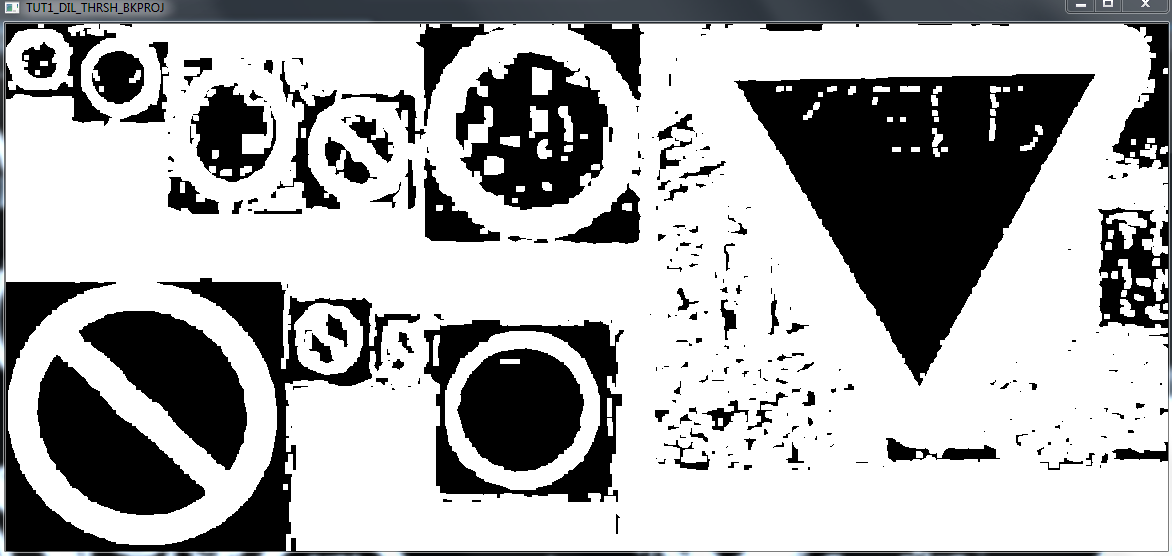
\includegraphics[width=0.9\linewidth, height=5cm]{N_DIL_THRESH_BKPROJ.PNG} 
\caption{The back projected image}
\label{fig:subim1}
\end{subfigure}
\begin{subfigure}{0.5\textwidth}

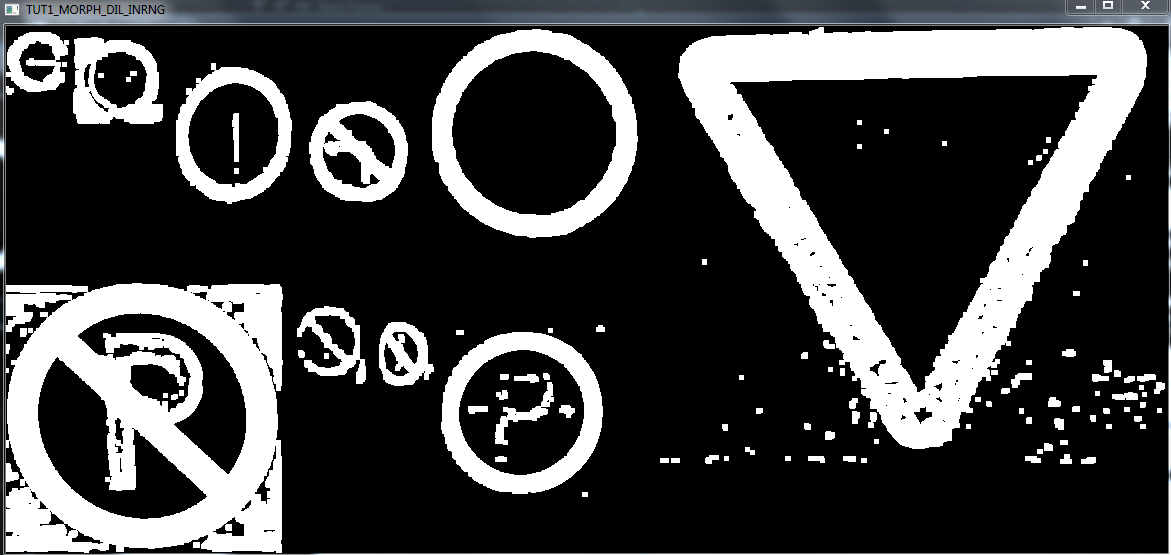
\includegraphics[width=0.9\linewidth, height=5cm]{N_MORPH_DIL_INRNG.PNG}
\caption{The inRange thresholded image}
\label{fig:subim2}
\end{subfigure}
\caption{Figure of constructed tresholded images}
\label{fig:image2}
\end{figure}

\begin{figure}[H]
\center
\begin{subfigure}{0.5\textwidth}
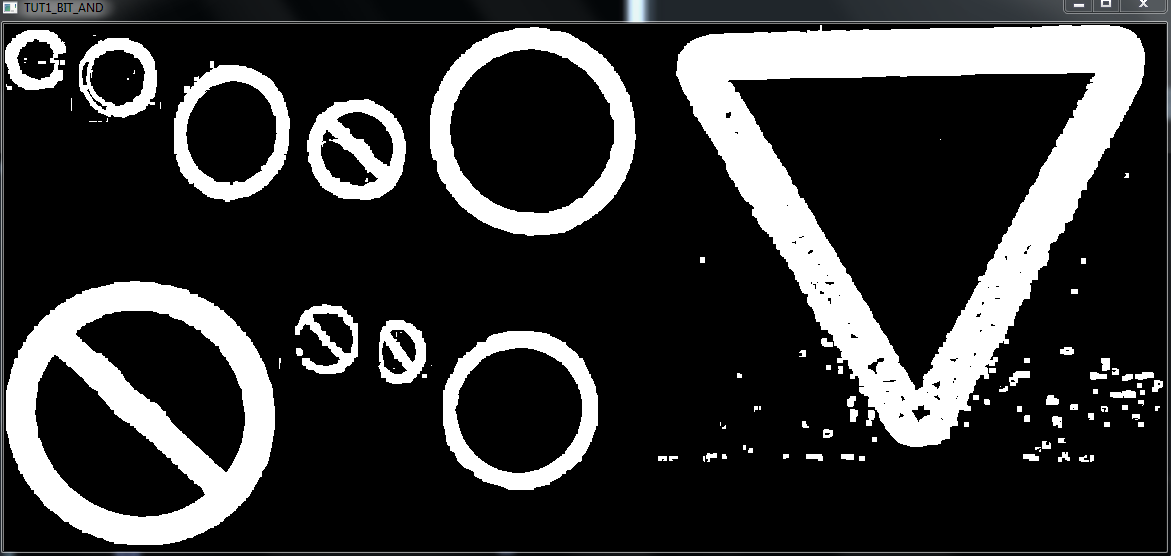
\includegraphics[width=0.9\linewidth, height=5cm]{N_BIT_AND.PNG} 
\caption{The two images above ANDed give this result}
\label{fig:subim1}
\end{subfigure}
\caption{Figure of constructed of the two tresholded images}
\label{fig:image2}
\end{figure}


\begin{lstlisting}
		inRange(hls_test, Scalar(10,10,55), Scalar(210, 190, 200), inrange_test);
		dilate(inrange_test, dil_inrange_test, Mat(), Point(-1, -1), 2, 1, 1);
		// Two images, back proj and inrange merged together
		bitwise_and(dil_thresh_backproj, morph_dil_inrange_test, band_rng_bkprj);
		dilate(band_rng_bkprj, band_rng_bkprj, Mat(), Point(-1, -1), 1, 1, 1);
		/*Dilate and morphology again to close the remaining gaps*/
		morphologyEx(band_rng_bkprj, band_rng_bkprj, MORPH_TOPHAT, element, Point(-1, -1), 50);
		bitwise_and(roadsign_test,roadsign_test,redcrop, band_rng_bkprj);
\end{lstlisting}
The code above shows how inRange was used to get a similar but different thresholded image which has fuller contour of the road sign pictures but also a lot of other false positive shapes. The thresholded image was also somewhat inaccurate, but by merging the two pictures  together using AND a much clearer and more accurate representation of the red pixels in the image would be achieved. The image was then dilated and closed to help with remaining holes and breaks in the shapes. Finally the resulting image was used as a mask to construct a composite image to show how much of the red pixels from the original image were captured.

\begin{figure}[H]
\begin{subfigure}{0.5\textwidth}
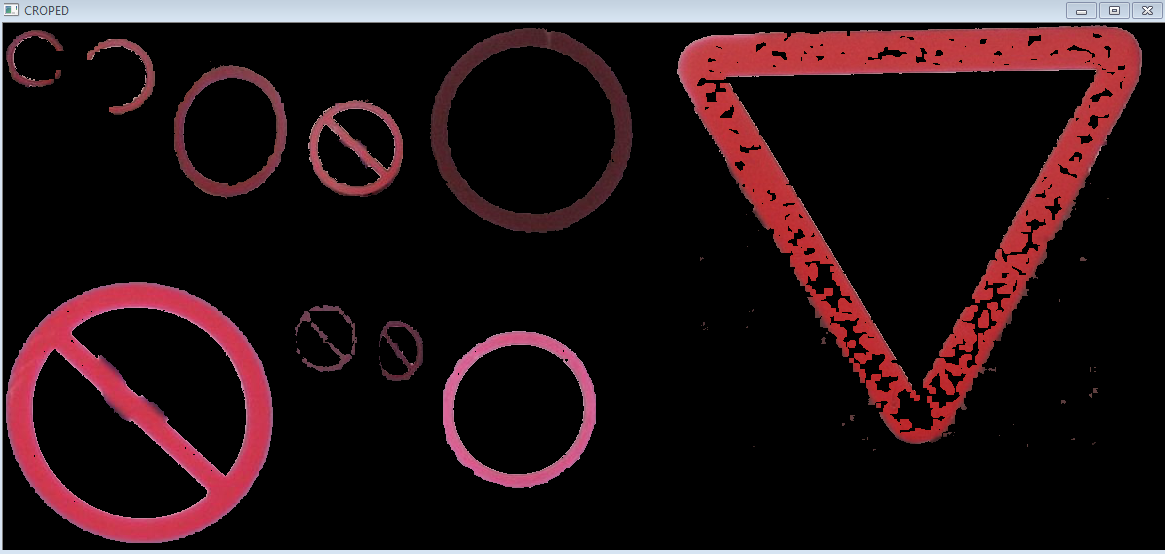
\includegraphics[width=0.9\linewidth, height=5cm]{CROPP.PNG} 
\caption{A previous, less succesfull composite image using the previous $($a$)$ red sample image}
\label{fig:subim1}
\end{subfigure}
\begin{subfigure}{0.5\textwidth}
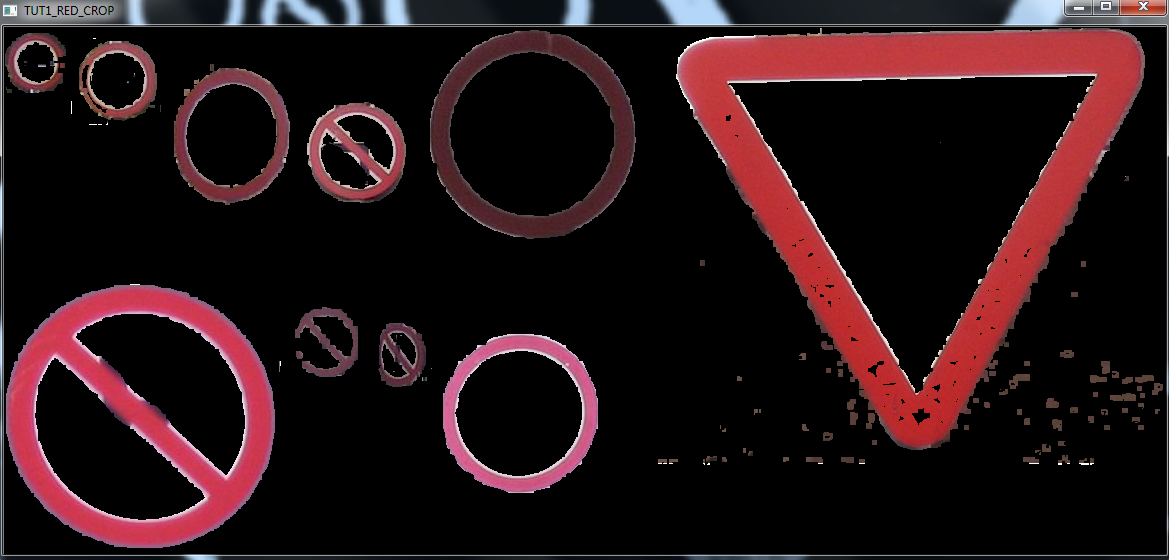
\includegraphics[width=0.9\linewidth, height=5cm]{N_RED_CROP.PNG}
\caption{The composite image showing the current red mixels detected}
\label{fig:subim2}
\end{subfigure}
\caption{Figure of constructed tresholded images}
\label{fig:image2}
\end{figure}




\begin{lstlisting}
CompareRecognitionResults(band_rng_bkprj, ground_red);
\end{lstlisting}
The above code shows the use of the function CompareRecognitionResults to compare the example thresholded red pixel image with the thresholded ground pixel image to achieve a score for the performance method. \\
The ground image is converted to HLS and then used inRange on it as discussed before. The only difference to this is that the ground image has only one overall value for each color present, making it very easy to threshold out the colors. Thus the following code was used to get the ground thresholded images of the three colors.
\begin{lstlisting}
	inRange(hls_ground, Scalar(0, 0, 255), Scalar(0, 0, 255), ground_white);
	inRange(hls_ground, Scalar(0, 255, 255), Scalar(0, 255, 255), ground_red);
	inRange(hls_ground, Scalar(0, 0, 0), Scalar(0, 0, 0), ground_black);
\end{lstlisting}
%\includegraphics[height=2in,width=5in]{}
%\includegraphics[height=2in,width=5in]{}




\subsection{Performance}\label{sec:intro}
The performance of the thresholded image was tested using the function provided in the practice tutorial. As seen in the picture and table, the precision for the color red is lower than that of black or white pixels. This is due in part to the difficulty in constructing a red sample image for the histogram. The innacuracy is also due to the dilation used on the shapes to connect the circles. The methadology helped in improving black and white pixel detection but at the cost of decreasing red pixel detection precison.\\
As per the accepted definitions of accuracy and precision. The two are independent of each other. Thus a method can be neither precise nor acurate, precise and not accurate, accurate and not precise or for best results, accurate and precise.\\
Accuracy defines how close and measurement is to the standard or known value, thus the red sample values to the accepted red values. Precision defines how close  a measurement is to another measurement. Thus how close the red sample values were to the ground sample values.\\
Looking at the score for precision it is clear that this methadology was accurate but not very precise in determining the red pixels.\\

\begin{figure}[H]
\center
\begin{subfigure}{0.5\textwidth}
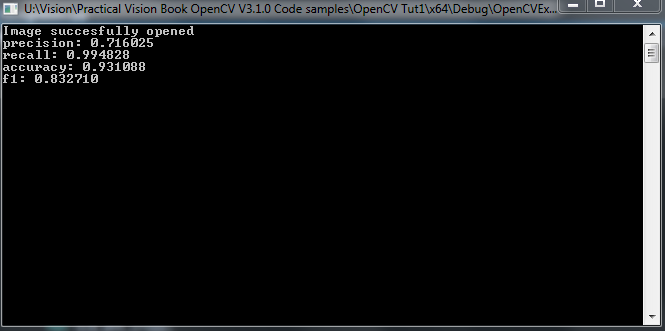
\includegraphics[width=0.9\linewidth, height=4cm]{N_RED_STAT.PNG} 
\caption{The image shows the scoring achieved for the red pixels}
\label{fig:subim2}
\end{subfigure}
\caption{The figure shows the scores for red pixel recognition}
\label{fig:image2}
\end{figure}

\begin{table}[]
\centering
\caption{RED PIXEL DETECTION VALUES}
\label{my-label}
\begin{tabular}{@{}|l|l|@{}}
\toprule
{\ul TYPE} & {\ul VALUE} \\ \midrule
Precision  & 0.716025    \\ \midrule
Recall     & 0.994828     \\ \midrule
Accuracy   & 0.931088    \\ \bottomrule
\end{tabular}
\end{table}


\subsection{Discussion}\label{sec:intro}
One of the earliest problems noticed with hand sampling the red from the road signs was that the quality of the pictures was quite low. The pictures were also taken at an angle and with different cameras, thus the sharpness of the image also varied from picture to picture. \\

The biggest problem with sampling the sample road signs image was the fact that a lot of the road signs had two, three or even more layers of shadowing on them. This created a problem which was only noticed when the process of constructing the sample image by busket fill in the various squares. I would, to my knowledge pick a red point in a sign only to discover that this point looked oddly brown or purple when transferred to my sample red image that was inserted into the histogram. These brown and purple points also caused a problem further down the road when dark bits of the background were identified as red due to those brownish squares.\\


The performance for red pixels detection is high although it could have been higher. One major obstacle in a more precise detection algorythm is the quality of the pictures themselfes. Another being the background of the picture. While performing this assignment I have found it quite diffucult to separate a red road sign from its red brick background. Should even more red objects had been present in the picture, a more advanced form of Canny would have to be used to separate the objects and only then perhaps perform back projection.\\


By observing the threshold images provided for red pixel detection it can be clearly noticed that the picture has false positives, where it recognized parts of the background building as parts of the road sign due to the closeness in hue. It also contains false negatives where, it did not recognize parts of the red borders in the road signs, possibly due to the color being altered by a shadow to a hue outside the target zone. These errors, which were due to the factors previously discussed, posed the biggest challenge to making an accurate and precise road sign detecting opencv program.\\



\pagebreak
\section{BLACK AND WHITE PIXEL DETECTION}
\subsection{Intro}\label{sec:intro}
In this section the procedure and results for detecting black and white pixels is outlined. The white and black pixels could not be thresholded like the red pixels for a number of reasons. White could not be thresholded due to it composing the majority of the background onto which all the sample road sign images were placed. The innacuracy would have been to great. Black could not be thresholded due to it again existing in other places than the inside of the road signs, again such a process would have induced too many false positives. Thus a contour hiararchy process had to be implemented.\\


\subsection{Procedure}\label{sec:intro}
To get the thresholded image of the white and black pixels a contour hierarchy process was used. Due to the previous red pixel detection process being altered, the thresholded red pixel road sign contours were closed shapes. Thus by using floodfilll, the inner space can be cropped away. Floodfill works by filling the inside of only closed border shapes in the red pixel thresholded image and then XORing the original red pixel thresholded image with the new flood filled inner image. The combination of these two images creates a composite which only has the inner space of the borders of the road signs in the thresholded red pixel image.\\
The problem now is that this image will encompass the white and black pixels inside the red border of the road sign. \\
\begin{figure}[H]
\begin{subfigure}{0.5\textwidth}
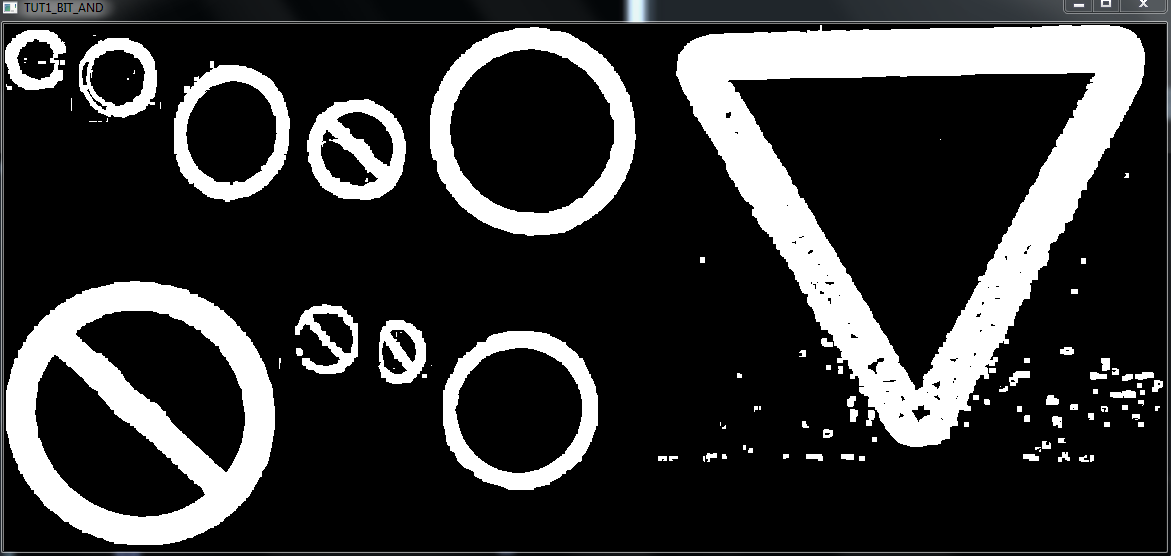
\includegraphics[width=0.9\linewidth, height=5cm]{N_BIT_AND.PNG} 
\caption{The composite thresholded image}
\label{fig:subim1}
\end{subfigure}
\begin{subfigure}{0.5\textwidth}
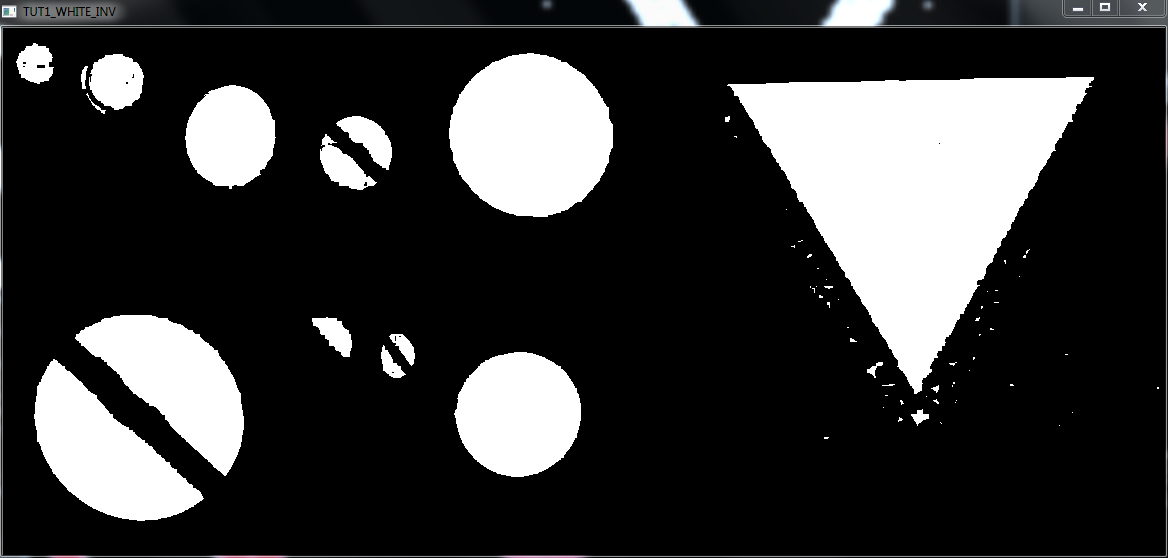
\includegraphics[width=0.9\linewidth, height=5cm]{N_WHITE_INV.PNG}
\caption{The floodfilled image}
\label{fig:subim2}
\end{subfigure}
\caption{The figure shows how floodfill works}
\label{fig:image2}
\end{figure}

\begin{figure}[H]
\center
\begin{subfigure}{0.5\textwidth}
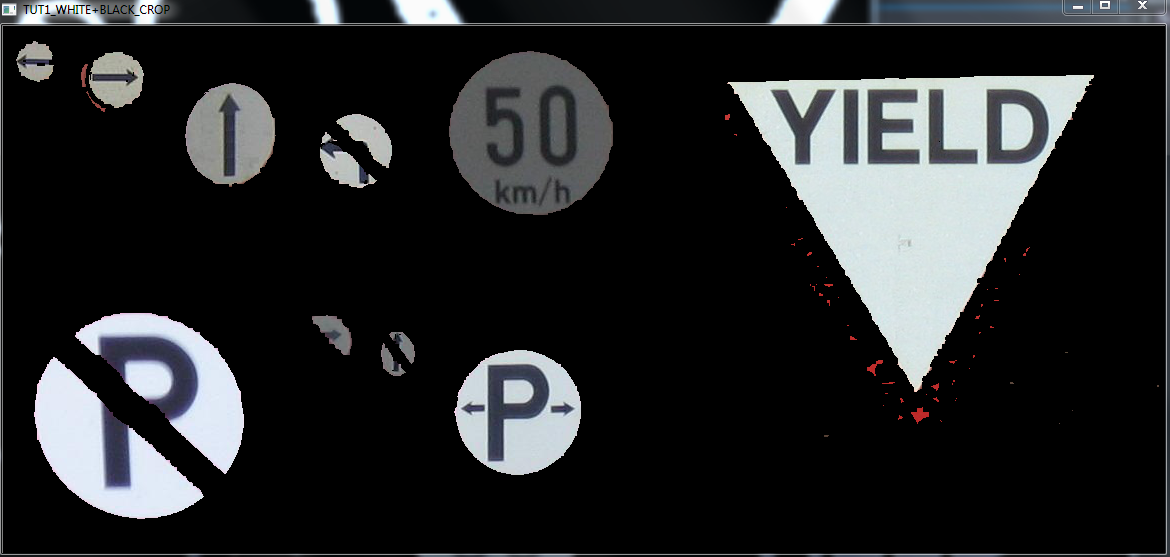
\includegraphics[width=0.9\linewidth, height=5cm]{N_BLACK+WHITE_CROP.PNG} 
\caption{The two images above show the process of the contour hiararchy. (b) is then used as a mask on the original color image to construct this new composite image}
\label{fig:subim1}
\end{subfigure}
\caption{The figure shows how the contour hierarchy works}
\label{fig:image2}
\end{figure}



\begin{lstlisting}
		bitwise_not(white_ff, white_ff_not);
		Mat white_out = (band_rng_bkprj | white_ff_not);
		bitwise_xor(band_rng_bkprj, white_out, whiten);
		bitwise_and(roadsign_test, roadsign_test, whiteblackcrop, whiten);
		cvtColor(whiteblackcrop, wbcgrey,CV_BGR2GRAY);
		threshold(wbcgrey, trsh_wht, 85, 255, CV_THRESH_BINARY);
		bitwise_and(roadsign_test, roadsign_test, cropp_white, trsh_wht);
\end{lstlisting}
To separate black from white the new image needs to be ANDed with the original color image to get the location of the white and black pixel placement. Once a composite is created it is then grayscaled and thresholded, this will result in a new image which will only have the white pixels present. 

\begin{figure}[H]
\begin{subfigure}{0.5\textwidth}
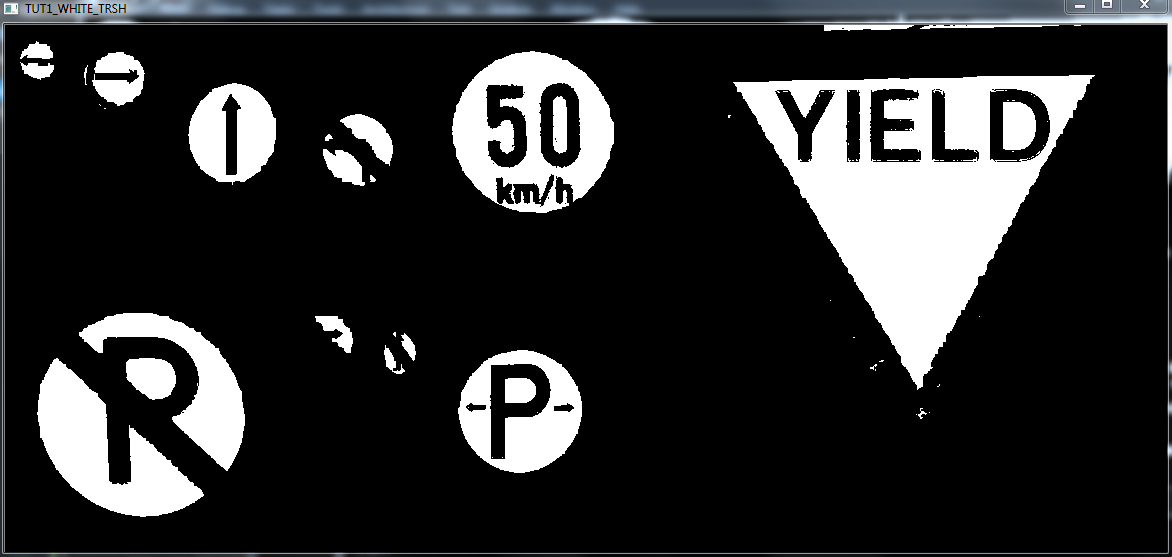
\includegraphics[width=0.9\linewidth, height=5cm]{N_WHT_TRSH3.PNG} 
\caption{The composite thresholded image to get only the white outline}
\label{fig:subim1}
\end{subfigure}
\begin{subfigure}{0.5\textwidth}

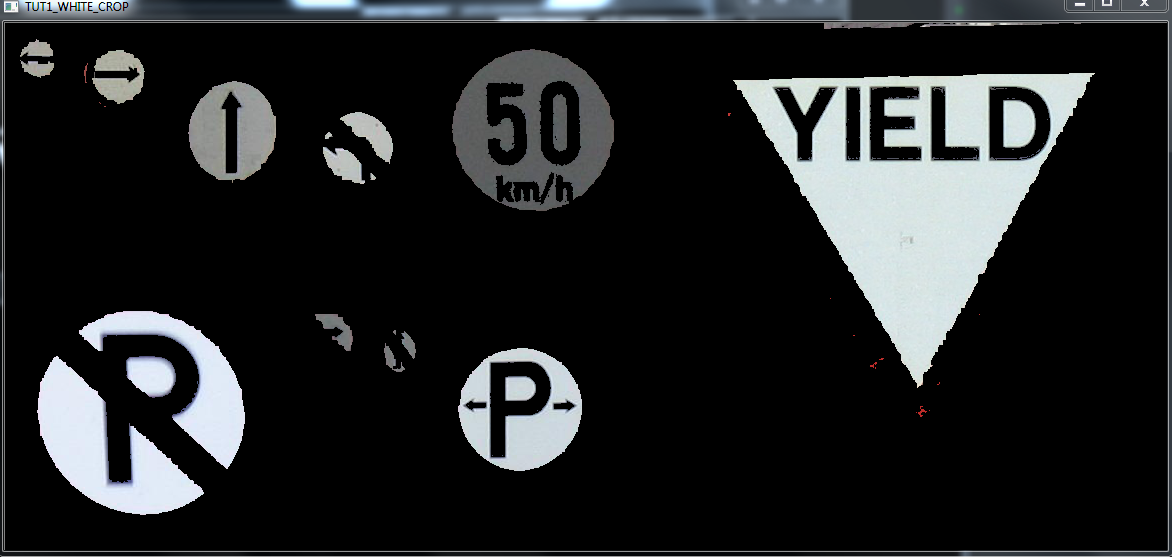
\includegraphics[width=0.9\linewidth, height=5cm]{N_WHITE_CROP3.PNG}
\caption{The image in $($a$)$ used as a mask on the original color image to show how much of the white pixels can be detected}
\label{fig:subim2}
\end{subfigure}
\caption{The figure shows how contour hierarchy can be used to section off the white pixels.}
\label{fig:image2}
\end{figure}


The inner thresholded image is grayscaled to help with the thresholding but also to convert it to the appropriate CV\underline{ }8UC1 format. If the image is not grayscaled the image matrix will be a different size than those of the ground image and thus will not be possible to be accurately compared, or as I found early on, to be even successfully inputted into the function.\\
\begin{lstlisting}
		Mat blk_ff = cropp_white.clone();
		floodFill(blk_ff, cv::Point(0, 0), Scalar(0,0,0));
		bitwise_not(blk_ff, blk_ff_not);
		bitwise_and(whiteblackcrop, blk_ff_not, blk_trsh );
		/*have to grayscale otherwise image format is not accepted*/
		cvtColor(blk_trsh, blk_trsh, CV_BGR2GRAY);
		threshold(blk_trsh, blk_trsh, 0, 255, CV_THRESH_BINARY);
\end{lstlisting}
To get a thresholded image of the black pixels the same process was repeated again. \\
Thus the white pixel thresholded image is XORed with the original black and white thresholded image, resulting in a composite image which has only the black road sign pixels sectioned off. This is then ANDed with the original color image, grayscaled so it has the appropriate format and thresholded again so that it can be inputted into the precision function.\\



\begin{figure}[H]
\begin{subfigure}{0.5\textwidth}
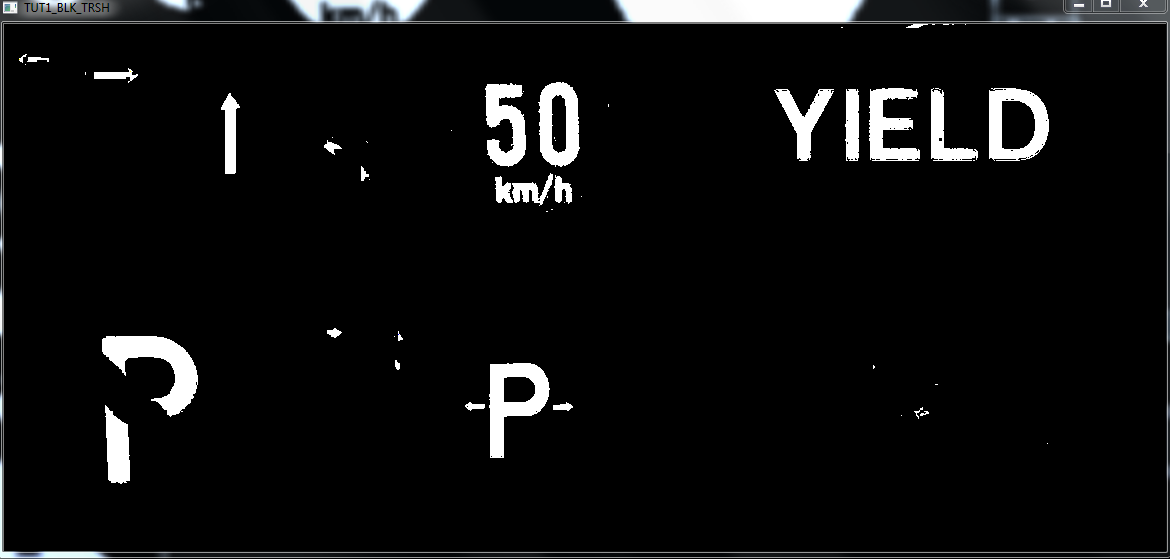
\includegraphics[width=0.9\linewidth, height=5cm]{N_BLK_TRSH.PNG} 
\caption{The composite thresholded image to get only the black pixels inside the road signs}
\label{fig:subim1}
\end{subfigure}
\begin{subfigure}{0.5\textwidth}
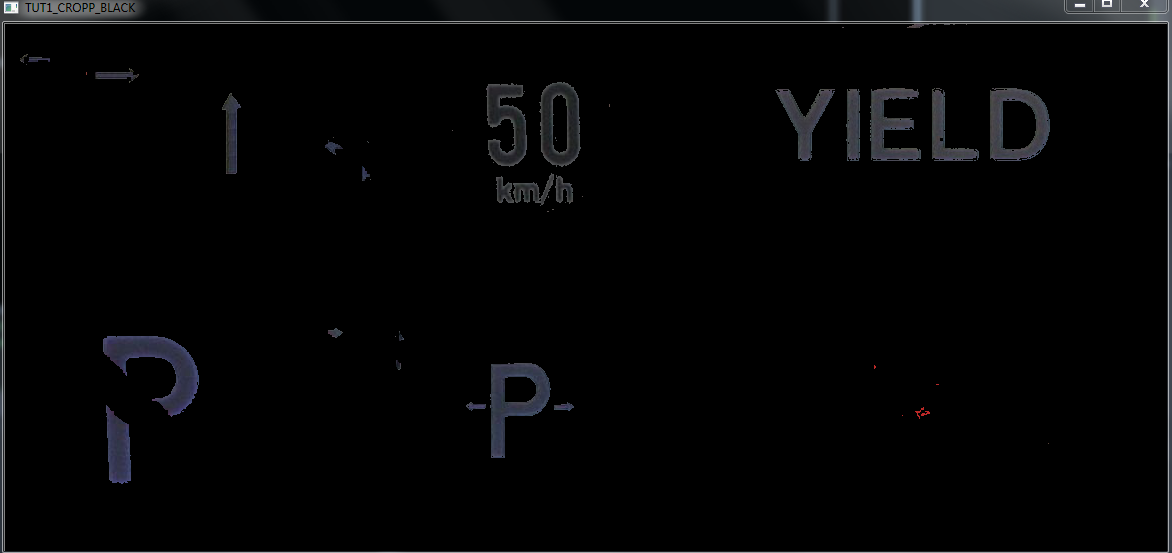
\includegraphics[width=0.9\linewidth, height=5cm]{N_BLK_CROPP.PNG}
\caption{The image in $($a$)$ used as a mask on the original color image to show how much of the black pixels can be detected}
\label{fig:subim2}
\end{subfigure}
\caption{The figure shows how contour hierarchy can be used to section off the black pixels inside the road signs.}
\label{fig:image2}
\end{figure}

\begin{lstlisting}
		CompareRecognitionResults(blk_trsh, ground_black);
		CompareRecognitionResults(scd_wht_cropp, ground_white);
		
\end{lstlisting}
The above code shows the last parts of the program in which the example thresholded images for white and black are compared with the thresholded images of the the ground image.
\subsection{Performance}\label{sec:intro}
The performance of the white and black pixels was deduced from inserting the thresholded white and black pixels images into the Recognition function previously specified. As can be seen from the tables and images provided the precision on both types of pixels was significantly higher than that of the red pixels.\\
The white pixels have the highest precision, this can be due to the fact that white is the easiest color to threshold out. The contour hiararchy process has thus proven that it is more accurate. One easy explination for such a high white pixel precision is that the white pixels had the least amount of variance between them. Thus the ground and sample white pixels were closer in hue range than the red pixels. The white pixels have a lower accuracy than the black pixels though. This again can be deducted from the false positives and false negatives present in the thresholded image.\\
The lower precision in blackpixels can be due to the fact that the thresholding process limitations may have been off, thus loosing some detail present in the process. It could also be due to the fact that the black pixels in the road sign were not pure black, just like the red a white, the black pixels had some lighter parts to them which may have been lost in the contour or thresholding processes. The higher accuracy in black could be due to black being easier to define than white.\\
In the contour hiararchy process, half a sign was lost, thus immediatelly adding a false negative to all images there after, it is more than probable that the missing sign is responsible for some loss of accuracy and precision. The other factor is that to maintain the rest of the signs through out the contour hiararchy process the contour borders were dilated thus false positives were also introduced in all subsequent images.

\begin{figure}[H]
\begin{subfigure}{0.5\textwidth}
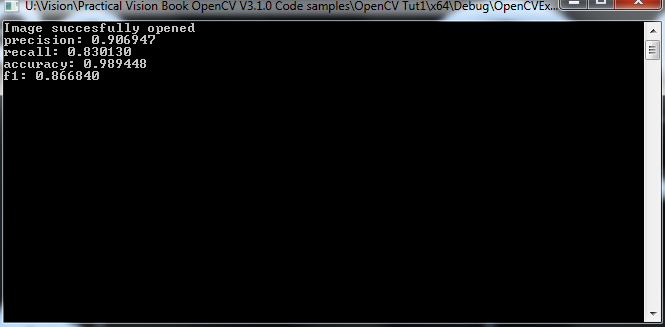
\includegraphics[width=0.9\linewidth, height=5cm]{N_BLK_STAT.PNG} 
\caption{The image shows the scoring ac hieved for the black pixels}
\label{fig:subim1}
\end{subfigure}
\begin{subfigure}{0.5\textwidth}
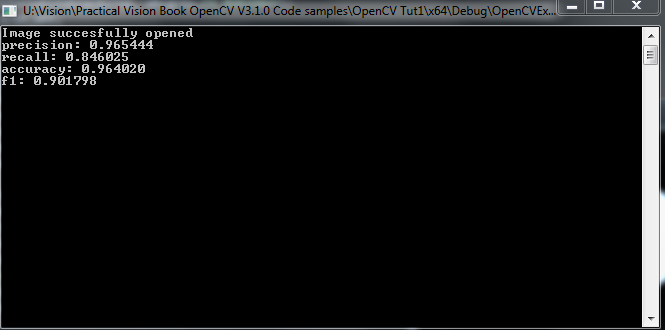
\includegraphics[width=0.9\linewidth, height=5cm]{N_WHT_STAT.PNG} 
\caption{The image shows the scoring ac hieved for the white pixels}
\label{fig:subim2}
\end{subfigure}
\caption{The figure shows the scores for the white and black pixel recognition}
\label{fig:image2}
\end{figure}

\begin{table}[H]
\centering
\caption{The figure shows the scores for white and black pixel recognition}
\label{my-label}
\begin{tabular}{@{}|l|l|l|l|l|@{}}
\cmidrule(r){1-2} \cmidrule(l){4-5}
{\ul TYPE} & {\ul WHITE VALUE} &  & {\ul TYPE} & {\ul BLACK VALUE} \\ \cmidrule(r){1-2} \cmidrule(l){4-5} 
Precision  &      0.965444       &  &    Precision        &  0.906947      \\ \cmidrule(r){1-2} \cmidrule(l){4-5} 
Recall     &      0.846025       &  &    Recall         &  0.830130     \\ \cmidrule(r){1-2} \cmidrule(l){4-5} 
Accuracy   &      0.964020       &  &    Accuracy         &  0.989448  \\ \cmidrule(r){1-2} \cmidrule(l){4-5} 
\end{tabular}
\end{table}

\pagebreak
\subsection{Discussion}\label{sec:intro}
The accuracy of the black and white pixels was somewhat a bit more accurate as there were far less similar background colors. Thus there was less interference and the background could be sectioned off more easily. The hue range to which the black and white pixels extended was also far narrower than that of the red pixels.\\
By taking a look at the thresholded images provided for black and white pixels it can be seen that many of them contain false negatives. The lower part of a sign had been lost in the tresholding process due to its borders not being fully closed during flood fill. \\
Lastly, the biggest issue I encountered during this assignment was the values by which to threshold, dilate and erode. Unlike other functions in opencv, these processes require a human opinion. During the thresholding processes I struggled to understand why one lower or higher limit is better than another. My only conclusion from this process is that at the end of the day opencv requires a human to truly define what is useful and what is not. The values therfore that I used for my thresholding process were my personal input for what would make an accurate program.\\
The theme of human assisted detection seems to be constant across all processes, from deceting a simple color to defining what is a border. This may have something to do with the fact that even the world we perceive is subject to our interpretations, thus vision itself can never be binary, in a sense that an answer is right or wrong. It will always lie within a spectrum of accuracy and precision dependent on subjective opinions.




\pagebreak
\end{document}


